\documentclass[10pt,letterpaper]{article}
\usepackage{fullpage}
\usepackage{xcolor}
\usepackage[top=1in, bottom=1in, left=1in, right=1in]{geometry}
\usepackage{graphicx}
\usepackage{wrapfig}
\usepackage{hyperref}
\usepackage{booktabs}
\usepackage{multirow}
\usepackage{amsmath}
\usepackage{subcaption}

\newcommand{\todo}[1]{\textcolor{red}{TODO:\ #1}}
\newcommand{\shortname}{EqMap}

\title{ECE6745 Project -- ASIC Technology Mapping with E-Graphs}
\author{Matthew Hofmann}
\date{\today}

\begin{document}

\maketitle

% Revised Sections
% Introduction
% Background (lit review)
% Baseline design

\section{Introduction}\label{sec:intro}
\subsection{Motivation}\label{sec:intro:motivation}

As the trends of transistor scaling come to a close, the QoR (quality of
results) of EDA tools will become more of a bottleneck in the hardware design
process. Given new developments in compiler technology and automated reasoning
tools, it is possible to better study the suboptimality of the EDA tool stack.
Several of the heuristics used in core EDA algorithms were invented decades
ago, and increases in compute capacity in the modern era afford us a more
formal and exploratory approach to optimizing digital logic. In this project, I
use the automated reasoning capabilities of equality graphs (e-graphs) to more
precisely explore optimal designs points in the PPA (power, performance, area)
trade-off space. With my results, I demonstrate that e-graph driven compilers
can better span the wide gap between SAT-based, exact synthesis and fully
heuristic algorithms.

\subsection{Project Proposal}\label{sec:intro:proposal}

Over the length of this course project, I have developed a tool which uses
e-graphs to superoptimize ASIC technology mapping. Besides developing the core
optimization and mapping framework, I have developed a Verilog parser and
emitter to be able to test my technique against existing RTL tools. In short, I
will be comparing against Synopsys Design Compiler. Across 96 RTL benchmarks,
my tool, called \shortname{}, should be able to more exactly synthesize
combinational logic to standard cells. My goal is roughly 10\% area savings
without increasing the circuit depth.

I am optimistic tat my tool can outperform Synopsys on small designs, because
e-graphs can explore circuit topologies that heuristic methods cannot. However,
the real challenge may lie in the extraction algorithm. For this reason, I will
also consider optimizing for delay if that proves to be more feasible than
optimizing for area. All of these experiments were relatively low cost to
start, because I have a lot of compiler infrastructure already built up. For
instance, I have a custom, bare-bones Verilog frontend. In the following
sections, I will give the literature review needed to understand equality
graphs for superoptimization as well as ASIC technology mapping in general.

\section{Literature Review}\label{sec:background}

\subsection{E-Graphs}\label{sec:background:egraph}

Equality graphs, most commonly referred to as \textit{e-graphs}, are an
automated reasoning tool built around a union-find data
structure~\cite{eggpaper}. An e-graph is essentially a directed graph with two
extra features: (1) nodes are grouped together into \textit{e-classes} and (2)
edges always start at a node and point to an e-class. As a consequence,
e-graphs can very compactly store a collection of equivalence relations. The
prototypical example for e-graphs involves the rewriting of arithmetic
expressions. For instance, one relation conveyed in Fig.~\ref{fig:egraph} is
that \texttt{a << 1} is equal to \texttt{a * 2}. To convey equality, the
anchoring nodes \texttt{<<} and \texttt{*} are grouped in the same e-class (the
dotted box). However, it is important to note that the destination of edges is
always an e-class and not a node. With this illustration, it hopefully becomes
clear why e-graphs are strong at equational reasoning.

\begin{wrapfigure}{r}{0.47\textwidth}
    \centering
    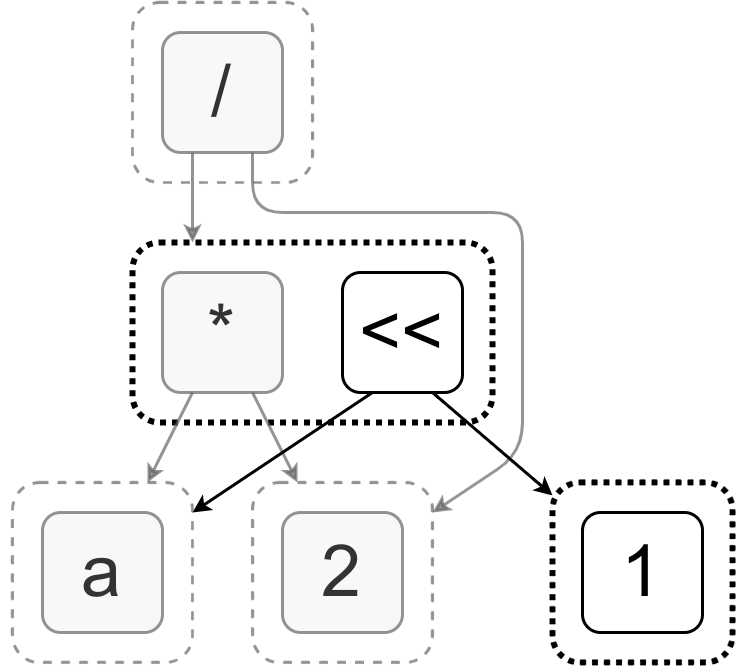
\includegraphics[width=0.44\textwidth]{img/egraph.png}
    \caption{An e-graph with 5 e-classes and 6 e-nodes.}\label{fig:egraph}
\end{wrapfigure}

To give some practical examples, e-graphs have been used to rewrite
mathematical expressions~\cite{egraphmath} or for automated reasoning about
functional programs~\cite{cclemma}. In the case of EDA software, e-graphs can
drive logic synthesis by exploring other circuit topologies. Initially, each
circuit node starts alone in its equivalence class. Then, a set of rewrite
rules is used to grow the e-graph with alternative representations. When
rewrite rules no longer introduce new information into the graph, we say we
have reached \textit{equality saturation}.

Of course, optimizing technology mapping for area is still an NP-hard problem.
E-graphs defer the difficult problem of finding the `best' circuit into a phase
called \textit{extraction}. This is where heuristics are re-introduced. There
are several research projects on e-graph
extraction~\cite{smoothe,sparsextract}, but they are beyond the scope of this
course project. However, previous work on FPGA technology mapping has
demonstrated that fast, greedy extraction algorithms can be used and still find
area and circuit depth improvements. Previous work~\cite{esyn} has demonstrated
the usefulness of e-graphs for logic synthesis. Moreover, I hope to submit my
own e-graph work to ICCAD which shows 12\% area savings over vendor tools on
FPGA applications without increasing circuit depth.

\subsection{ASIC Technology Mapping}\label{sec:background:techmapping}

The standard-cell design methodology for semiconductors came to fruition in the
1980s and 90s. While ASIC design as a general technique is more manageable than
full-custom layouts, there are still provably difficult problems in the flow.
In general, Boolean logic minimization is NP-hard, and this carries over to
more architecture-specific problems, like technology mapping. Technology
mapping is the compilation step which converts the abstract RTL logic into a
network of design elements that belong to the standard cell library. In other
words, the input is the user-written logic and the output is a gate netlist.
Since exact technology mapping is hard, most logic synthesis tools are largely
driven by heuristics---either for minimizing area or delay. For instance,
Lily~\cite{areamap} takes into account the connectivity of a circuit in order
to reduce area dedicated to routing signals. Another is example is
how~\cite{powermap} maps cells while taking into account signal transition
probabilities in order to minimize power. Recent developments include works
that use more approximate methods to drive synthesis. For example,
ALS~\cite{approxmap} uses reinforcement learning to do a form of `lossy' logic
synthesis. In my project, I will mostly perform area optimization by tracking
cell counts.

\section{Baseline Compiler Design}\label{sec:baseline}

In the initial design of the compiler, I have developed a logic rewriting
system and an extraction technique that can potentially achieve lower area than
Synopsys Design Compiler. In the case of FPGA technology mapping, I already
have results that show 12\% area savings over the vendor tools without
degrading timing. While greedy extraction shows promise for FPGA applications,
it may be that the same extraction algorithm will be less optimal for ASIC
design. Nonetheless, I anticipate that future work on e-graph extraction
algorithms will improve the circuit synthesis abilities without having to
update the rewriting system. Hence, the logic rewriting system proposed in this
work should be reusable in the future.

\subsection{Boolean Logic Rewriting}\label{sec:baseline:rewriting}
In any case, we can begin to break down the components of the \shortname{}
compiler. First, we need to define the intermediate representation of the
combinational logic that will be rewritten. We can use Backus-Naur form
(BNF)\footnote{\href{https://en.wikipedia.org/wiki/Backus\%E2\%80\%93Naur\_form}{https://en.wikipedia.org/wiki/Backus-Naur\_form}}
to very concisely define the grammar of our intermediate representation of
Boolean logic:

\begin{verbatim}
<Const> ::= false | true

<Input> ::= <String>

<StdCell> ::= NAND_X1 | NOR_X1 | XOR2_X1 | ...

<Node> ::= <Const> | <Input> | (INV <Node>) | (AND <Node> <Node>) | (OR <Node> <Node>)
           | (<StdCell> <Node> <Node>) | (<StdCell> <Node> <Node> <Node>) | ...
\end{verbatim}

Given this very simple language, we can represent any Boolean circuit we want.
For example, we could represent a 2:1 multiplexer with the following syntax:
\texttt{(OR (AND a s) (AND b (INV s)))}. Given this language with formal
semantics, we can write all the properties of Boolean algebras as rewrite
rules. Table.~\ref{tab:rules} shows that there are 19 logic rewriting rules in
total. For more information on the completeness of these rules, one should read
more into the axiomatization of Boolean algebras
\footnote{\href{https://en.wikipedia.org/wiki/Boolean\_algebra\_(structure)\#Axiomatics}{https://en.wikipedia.org/wiki/Boolean\_algebra\_(structure)\#Axiomatics}}.

\begin{table}[h]
    \centering
    \begin{tabular}{cl}
        \toprule
        \textbf{Property}                 & \textbf{Rules}                                         \\ \midrule
        \multirow{2}{*}{Short-Circuit}    & \texttt{(OR a true) => true}                           \\
                                          & \texttt{(AND a false) => false}                        \\ \midrule
        \multirow{2}{*}{Annulment}        & \texttt{(OR a false) => a}                             \\
                                          & \texttt{(AND a true) => a}                             \\ \midrule
        \multirow{2}{*}{Commutativity}    & \texttt{(OR a b) => (OR b a)}                          \\
                                          & \texttt{(AND a b) => (AND b a)}                        \\ \midrule
        \multirow{2}{*}{Associativity}    & \texttt{(OR (OR a b) c) => (OR a (OR b c))}            \\
                                          & \texttt{(AND (AND a b) c) => (AND a (AND b c))}        \\ \midrule
        \multirow{2}{*}{Distributivity}   & \texttt{(OR a (AND b c)) <=> (AND (OR a b) (OR a c))}  \\
                                          & \texttt{(AND a (OR b c)) <=> (OR (AND a b) (AND a c))} \\ \midrule
        \multirow{2}{*}{Complement}       & \texttt{(OR a (INV a)) => true}                        \\
                                          & \texttt{(AND a (INV a)) => false}                      \\ \midrule
        \multirow{2}{*}{De Morgan's Laws} & \texttt{(INV (AND a b)) <=> (OR (INV a) (INV b))}      \\
                                          & \texttt{(INV (OR a b)) <=> (AND (INV a) (INV b))}      \\ \midrule
        \multirow{2}{*}{Idempotence}      & \texttt{(OR a a) => a}                                 \\
                                          & \texttt{(AND a a) => a}                                \\ \midrule
        \multirow{2}{*}{Absorption}       & \texttt{(OR a (AND a b)) => a}                         \\
                                          & \texttt{(AND a (OR a b)) => a}                         \\ \midrule
        Negation                          & \texttt{a => (INV (INV a))}                            \\
        \bottomrule
    \end{tabular}
    \caption{Rules of a Boolean algebra for EqMap}\label{tab:rules}
\end{table}

\subsection{Mapping to Gates}\label{sec:baseline:mapping}

Now that the compiler can reason about Boolean logic, it also needs to know how
to cover the logic with standard cells. We can do this in an ad-hoc fashion by
using rewrite rules to match to syntactical elements in the logic. For example,
the rule \texttt{(INV (AND a b)) => (NAND\_X1 a b)} denotes the logic function
of \texttt{NAND\_X1} and hence declares what portions of the graph it can
cover. Combining cell mapping with the rules from
Sec.~\ref{sec:baseline:rewriting} means that the e-graph will reason about
logic rewriting and mapping to standard cells simultaneously. Hence, the
e-graph can reason about many alternative mappings in parallel. Of course, the
primary trade-off is the memory and execution time needed to build the e-graph.
In any case, Table~\ref{tab:cells} contains an incomplete list of standard
cells and their logic functions in terms of the EqMap intermediate language.

\begin{table}[h]
    \centering
    \begin{tabular}{ll}
        \toprule
        \textbf{Logic Function}                       & \textbf{Standard Cell}                                             \\ \midrule
        \texttt{(INV a)}                              & \texttt{INV\_X1}, \texttt{INV\_X2}, \texttt{INV\_X4}, \ldots       \\
        \texttt{(INV (AND a b))}                      & \texttt{NAND2\_X1}, \texttt{NAND2\_X2}, \texttt{NAND2\_X4}, \ldots \\
        \texttt{(INV (OR a b))}                       & \texttt{NOR2\_X1}, \texttt{NOR2\_X2}, \texttt{NOR2\_X4}, \ldots    \\
        \texttt{(INV (AND (AND a b) (AND c d)))}      & \texttt{NAND4\_X1}, \texttt{NAND4\_X2}, \texttt{NAND4\_X4}, \ldots \\
        \texttt{(OR (AND b (INV a)) (AND a (INV b)))} & \texttt{XOR2\_X1}, \texttt{XOR2\_X2}, \texttt{XOR2\_X4}, \ldots    \\
        \texttt{(INV (OR (AND a b) c))}               & \texttt{AOI21\_X1}, \texttt{AOI21\_X2}, \texttt{AOI21\_X4}, \ldots \\
        \texttt{(INV (AND (OR a b) c))}               & \texttt{OAI21\_X1}, \texttt{OAI21\_X2}, \texttt{OAI21\_X4}, \ldots \\
        \bottomrule
    \end{tabular}
    \caption{An incomplete table of cells defined as rewrite rules}\label{tab:cells}
\end{table}

\begin{wrapfigure}{r}{0.47\textwidth}
    \vspace{-1cm}
    \centering
    \includegraphics[width=0.44\textwidth]{img/celllang.pdf}
    \caption{The compilation steps internal to \shortname{} Verilog tool.}\label{fig:flow:egraph}
\end{wrapfigure}

\subsection{Standard Cell Extraction}\label{sec:baseline:extraction}
Ideally, the e-graph is grown until rewrites no longer introduce new terms into
the graph. In the literature, this is called \textit{equality saturation}. In
practice, equality saturation takes too long, and empirically it is not
required to capture the majority of the optimization potential. The quality of
results are more so dependent on the extraction technique used. As explained in
Sec.~\ref{sec:background:egraph}, \textit{extraction} is the process of
selecting the ``best'' circuit from the e-graph. Given that e-graph can easily
contain hundreds of thousands of e-nodes across tens of thousands of e-classes,
a greedy extraction algorithm is the most pragmatic. The greedy extractor
iterates over the e-classes, updating the cost of the cheapest e-node until the
database of costs no longer change. In the baseline compiler, the cost model
simply counts the number of cells required to implement a logic function. For a
circuit node \texttt{x}, its cost is defined as follows:

\begin{figure}[h]
    \[
        F(\texttt{x}) = \begin{cases}
            0                                         & \text{if \texttt{x} is an \texttt{Input} or \texttt{Const}}        \\
            1 + \sum_{\texttt{c} \in C} F(\texttt{c}) & \text{if \texttt{x} is a standard cell with a set of children } C, \\
            \infty                                    & \text{if \texttt{x} is a not a \texttt{StdCell}}.
        \end{cases}
    \]
    \caption{The cost function is defined recursively. The \texttt{INV}, \texttt{AND}, \texttt{OR} node types are purely for logic rewriting, and hence have a cost of infinity to facilitate filtering these choices out of extraction.}\label{fig:cost}
\end{figure}

\subsection{Verilog Integration}\label{sec:baseline:backend}

In order to run meaningful experiments with \shortname{}, I needed to be able
to interface with existing RTL tool flows. This means building some sort of
Verilog compiler from scratch. A half-baked attempt may use a separate tool to
convert the Verilog to a more primitive format---perhaps an and-inverter graph
(AIG). However, if we want a high performance tool it is very important that
all compilation stages stay in DRAM. For example, some Verilog test cases are
50,000 lines of code. If we have multiple stages of serialization and parsing,
the performance of the compiler is doomed.

As a starting point, I use the \texttt{sv-parser} Rust crate. This parses the
Verilog and returns an abstract syntax tree (AST). Obviously, reusing a
full-featured Verilog parser is a tremendous amount of work saved. Nonetheless,
an AST is still far from having a compiled Verilog circuit. The AST simply
represents the structure of the input language, not the digital circuit itself.
All that is to say that compiling from an AST data structure is still a lot of
work. In total, I have around 2,000 lines of code dedicated to Verilog
compilation and emission. The entire codebase is creeping into 10,000 lines of
code. Fig.~\ref{fig:flow:egraph} shows the core steps of the compiler. First,
Verilog is compiled to the intermediate representation defined in
Sec.~\ref{sec:baseline:rewriting}. Then, the e-graph is generated with the
rewrite rules. Finally, the `best' circuit is extracted with the cost function
from Fig.~\ref{fig:cost} and it is converted back to Verilog. This enables
nearly seamless integration with other RTL-based tool flows.

\begin{figure}[h]
    \begin{subfigure}{\textwidth}
        \centering
        \includegraphics[width=\textwidth]{img/gates.pdf}
        \caption{The result when mapping a 2-bit CLA to gates of fan-in 2}\label{fig:test:gates}
    \end{subfigure}\vspace{0.5cm}
    \begin{subfigure}{\textwidth}
        \centering
        \includegraphics[width=0.75\textwidth]{img/cells.pdf}
        \caption{EqMap reduces the cell count from 10 to 6 when OAI cells are introduced}\label{fig:test:cells}
    \end{subfigure}
    \caption{Diagrams of the top-level integration of \shortname{} into existing tool flows and internal e-graph driven compiler architecture.}\label{fig:flow}
\end{figure}

Since building out the compiler is the first priority, very little evaluation
was performed at this point. However, I can report the results of compiling one
example: a 2-bit carry lookahead unit. Part of the advantage of EqMap is the
flexibility of choosing which library to map to. For example,
Fig.~\ref{fig:test:cells} shows the advantage of introducing OAI and AOI cells
into the library. The mapping uses four less cells than
Fig.~\ref{fig:test:gates}.

\section{Alternative Compiler Design}\label{sec:alt}

\subsection{More Cells}\label{sec:alt:cells}

\begin{itemize}
    \item There are many alternate version of AOI and OAI gates, ranging from 3 to 5
          inputs
    \item Full adders and half adders.
    \item MUX2 and MUX4 cells.
    \item Majority gates.
\end{itemize}

\subsection{Heuristics Supplanted by Automated Reasoning}\label{sec:alt:heuristics}

\section{Testing}\label{sec:testing}

In the development of this tool, I used a varied testing strategy on both the
software development front and the circuit verification front. For the project
to be successful, it is very important to abstract the components of the
compiler wisely and test them rigorously. This enforces some level of
self-consistency in how the layers of the compiler integrate with each other.
Still, end-to-end testing is still required to capture the demands of the end
application---having a working Verilog-to-Verilog compiler. Hence, there is
nearly as much testing code as there is compiler code. The full list of testing
strategies is itemized below:

\begin{itemize}
    \item Software Testing
          \begin{itemize}
              \item Unit tests are written with the Rust Cargo tools in mind (\texttt{cargo test}).
              \item 36 end-to-end regression tests are ran with the full Verilog tool flow.
              \item Both of these test types are checked in a GitHub CI workflow.
              \item Results for 99 Verilog benchmarks are continually recorded and new commits are
                    checked for abnormalities.
              \item I self-enforce 80\% code coverage by line on my code.
          \end{itemize}
    \item Circuit Verification
          \begin{itemize}
              \item The intermediate language is its own statically typed data structure. A
                    mini-linter is built around it to check for syntax errors.
              \item The compiler performs exhaustive testing of combinational logic. Although, this
                    is only feasible for small circuits.
              \item Yosys RTL equivalence checking is used as a third party source to verify the
                    correctness of the Verilog output against the original Verilog input.
              \item The e-graph can produce a proof of the rewrite sequence that relates the
                    optimized and original form of the Verilog.
          \end{itemize}
\end{itemize}

\nocite{*}
\bibliographystyle{plain-annote}
\bibliography{references}

\end{document}